\chapter{力学经典题目}
\section{相对运动}
这一节是运动学的进一步深化,有助于同学们对运动学和力学的理解.其最典型的应用就是板块模型,这一节先来介绍相对运动.

\subsection{伽利略变换}

当一个物体被选为参考系时,此物体就应当认为是不动的,而研究其它的物体\CJKunderwave{相对于它}的运动.例如,物体$A$ 和 $B$ 分别\CJKunderwave{相对于地}运动,则如果将参考系选择为$A$ 则研究$B$ 相对于$A$ 的运动.

设物体$O$为参考系,$O'$在$O$系中运动,$O'$沿$O$的$x$轴运动,其位移为$x^*$,速度$v^*$,加速度$a^*$,其分别称为牵连位移,牵连速度,牵连加速度.同时有一个质点$A$也相对于$O$运动,在$O$系看来,质点$A$运动所需时间为$t$,位移为$x$,速度为$v$,加速度为$a$,则伽利略变换研究在$O'$中,质点$A$的时间$t'$,位移$x'$,速度$v'$和加速度$a'$的关系.

在经典力学中,认光传播的速度是无限大的,所以从$O$系到$O'$系经历的时间是相同的,即:$t'=t$.同时据图\ref{fig:xiangduiyundongx}所示,由几何关系可得$x'=x-x^*$
\begin{figure}[H]
  \centering
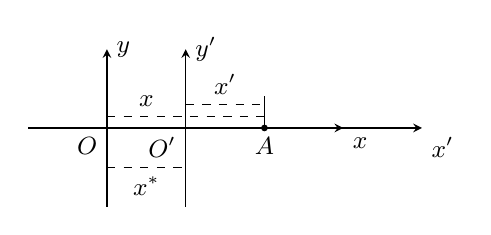
\begin{tikzpicture}
  \draw[->,>=stealth] (-1,0)--(3,0) node [anchor=north west]{\small $x$}; 
  \draw[->,>=stealth] (0,-1)--(0,1) node [anchor=west] {\small $y$}; 
  \draw (0,0) node [anchor=north east ] {\small $O$};
  \draw[->,>=stealth] (0,0)--(4,0) node [anchor=north west]{\small $x'$}; 
  \draw[->,>=stealth] (1,-1)--(1,1) node [anchor=west] {\small $y'$}; 
  \draw (1,0) node [anchor=north east ] {\small $O'$};
  \filldraw[color=black] (2,0) node [anchor=north] {\small $A$} circle [radius=1pt];
  \draw (2,0)--(2,0.4);
  \draw [dashed] (1,0.3)--(2,0.3);
  \draw (1.5,0.3) node [anchor=south] {\small $x'$};
  \draw [dashed] (0,0.15)--(2,0.15);
  \draw (0.5,0.15) node [anchor=south] {\small $x$};
  \draw [dashed] (0,-0.5)--(1,-0.5);
  \draw (0.5,-0.5) node [anchor=north] {\small $x^*$};
\end{tikzpicture}
  \caption{相对运动位移关系}
  \label{fig:xiangduiyundongx}
\end{figure}


  由此可得,经典绝对时空观下的伽利略变换\footnote{按照目前物理学的理解,正确的时空观应该是相对论时空观,其对应洛仑兹变换.经典时空观的伽利略变换可以认为是物体在低速运动时$\frac{v}{c}\to 0$ (c为光速,$c=3.0\times 10^8m/s$)的极限情况.}为
\begin{gather}
  t'=t\\
  x'=x-x^*
  \intertext{由速度的定义$v=\frac{\Delta x}{\Delta t}$可得}
  \frac{\Delta x'}{\Delta t}=\frac{\Delta x}{\Delta t}-\frac{\Delta x^*}{\Delta t}
  \intertext{即}
     v'=v-v^*
  \intertext{由加速度的定义$a=\frac{\Delta v}{\Delta t}$可得}
  \frac{\Delta v'}{\Delta t}=\frac{\Delta v}{\Delta t}-\frac{\Delta v^*}{\Delta t}
  \intertext{即}
     a'=a-a^*
\end{gather}

\section{板块模型}
这一节分别从绝对坐标系和相对坐标系下解决板块问题,请同学位认真体会,灵活运用.板块问题的核心是判断木块相对于木板运动的条件,如果板块间的静摩擦力达到最大值,则木块的加速度也就达到了最大,同时这也是板块一块运动最大加速度,一旦超过这个值则板块间将发现相对运动,下面具体分析.

\begin{calculate}
 1.如<:
 \begin{tikzpicture}
   \draw[color=white,pattern=north west lines](-2,0) rectangle (2,-0.2); 
   \draw (-2,0)--(2,0);
   \draw (-1.5,0) rectangle (1.5,0.2);
   \draw (-0.3,0.2) rectangle (0,0.5);
   \draw (-0.15,0.5) node [anchor=south]{\small B};
   \draw (-1.3,0.2) node [anchor=south]{\small A};
   \draw[->,>=stealth] (1.5,0.1)--(2.5,0.1) node [anchor=south east]{\small F};
 \end{tikzpicture}
 :>所示,厚度不计的薄板$A$长$l=5m$,质量$M=5kg$,放在水平地面上.在$A$ 上距右端$x=3m$ 处放一物体$B$ (大小不计),其质量$m=2kg$,已知$A$ 、$B$ 间的动摩擦因数$\mu_1=0.1$,$A$ 与地面间的动摩擦因数$\mu_2=0.2$,原来系统静止.现在板的右端施加一大小恒定的水平力$F=26N$,持续作用在$A$ 上,将$A$从$B$下抽出.$g=10m/s^2$,求:
 [1]$A$从$B$下抽出前$A$、$B$的加速度各是多大;
 [2]$B$运动多长时间离开$A$.

a.(1) $A$ 的加速度是$2m/s^2$ .$B$的加速度是$1m/s^2$\\
(2) $B$运动$\sqrt{10}s$离开$A$.

e.(1)对B受力分析如<:
 \begin{tikzpicture}
   \draw[color=white,pattern=north west lines](-2,0) rectangle (2,-0.2); 
   \draw (-2,0)--(2,0);
   \draw (-1.5,0) rectangle (1.5,0.2);
   \draw (-0.3,0.2) rectangle (0,0.5);
   \draw (-0.15,0.5) node [anchor=south]{\small B};
   \draw (-1.3,0.2) node [anchor=south]{\small A};
   \draw[->,>=stealth] (-0.15,0.35)--+(0,-1) node [anchor=west] {\small $mg$};
   \draw[->,>=stealth] (-0.15,0.35)--+(0,1) node [anchor=west] {\small $F_N$};
   \draw[->,>=stealth] (-0.15,0.35)--+(1,0) node [anchor=west] {\small $f$};
   \filldraw[color=black] (-0.15,0.35) circle [radius=1pt];
 \end{tikzpicture}
:>所示,由竖直方向平衡可得
$$F_N-mg=0$$
同时$f=\mu_1 F_N$,由牛顿第二定律得
$$\mu_1 mg = ma_B$$
解得
$$a_B=\mu_1g=1m/s^2$$

ee.对A受力分析如<:
 \begin{tikzpicture}
   \draw[color=white,pattern=north west lines](-2,0) rectangle (2,-0.2); 
   \draw (-2,0)--(2,0);
   \draw (-1.5,0) rectangle (1.5,0.2);
   \draw (-0.3,0.2) rectangle (0,0.5);
   \draw (-0.15,0.5) node [anchor=south]{\small B};
   \draw (-1.3,0.2) node [anchor=south]{\small A};
   \draw[->,>=stealth] (0,0.1)--+(0,-1.5) node [anchor=west] {\small $Mg$};
   \draw[->,>=stealth] (0,0.1)--+(0,-1) node [anchor=west] {\small $F_N'$};
   \draw[->,>=stealth] (0,0.1)--+(0,1) node [anchor=west] {\small $N$};
   \draw[->,>=stealth] (0,0.1)--+(-1,0) node [anchor=south] {\small $f'$};
   \draw[->,>=stealth] (0,0.1)--+(-1.5,0) node [anchor=east] {\small $F_f$};
   \draw[->,>=stealth] (0,0.1)--+(1.5,0) node [anchor=south] {\small $F$};
   \filldraw[color=black] (0,0.1) circle [radius=1pt];
 \end{tikzpicture}
:>所示,由牛顿第三定律得
$$F_N'=F_N=mg$$
$$f'=f=\mu_1mg$$
竖直方向受力平衡可得
$$N-F_N'-Mg=0$$
解得
$$N=(m+M)g$$
水平方向由牛顿第二定律得
$$F-\mu_2 N -f'=Ma_A$$
解得
$$a_A=\frac{F-\mu_2 (m+M)g-\mu_1mg}{M}=2m/s^2$$

ee.(2)首先讨论在\CJKunderwave{绝对坐标系}中解决问题.选择$A$点左端为原点,则木板$t$时刻的坐标为
$$x_A=\frac{1}{2}a_At^2$$
则物块$B$,在$t$时刻的坐标是
$$x_B=l+\frac{1}{2}a_Bt^2$$
$A$和$B$在$t$时刻的相对的距离为
$$\Delta x=x_B-x_A$$
代入$x_A$ 和 $x_B$ 的表达式得
$$\Delta x=l+\frac{1}{2}(a_B-a_A)t^2$$
当$B$从$A$上恰好掉下来时$\Delta x=0$,解得
$$t=\sqrt{\frac{2l}{a_A-a_B}}=\sqrt{10}s$$

ee.其次从\CJKunderwave{相对运动}的角度来考虑问题.选择$A$为研究对象,则$B$相对$A$的初速度为$0$,相对加速度为
$$a=a_B-a_A=-1m/s^2$$
当$B$从$A$上下刚刚下落时,$B$相对于$A$的位移为
$$x=-l=-5m$$
在以$B$为参考系的坐标系上来看,$B$向左做加速度大小为$1m/s^2$的匀加速直线运动,于是
$$x=\frac{1}{2}at^2$$
解得
$$t=\sqrt{\frac{2x}{a}}=\sqrt{\frac{2\times (-5)}{-1}}s=\sqrt{10}s$$

2.如<:
\begin{tikzpicture}
  \draw [color=white,pattern=north west lines] (-2,0) rectangle (2,-0.2);
  \draw (-2,0)--(2,0);
  \draw (-1.5,0) rectangle (1.5,0.2);
  \draw (0,0.1) node {\tiny M};
  \draw (-1.5,0.2) rectangle (-1.1,0.6);
  \draw (-1.3,0.4) node {\tiny m};
  \draw[->,>=stealth] (-1.1,0.4)--+(1,0) node [anchor=west]{\tiny F};
\end{tikzpicture}
:>所示,长度$l=2m$,质量$M=\frac{2}{3}kg$ 的木板置于光滑的水平地面上,质量$m=2kg$的小物块(可视为质点)位于木板的左端,木板和小物块间的动摩擦因数$\mu=0.1$,现对小物块施加一水平向右的恒力$F=10N$,取$g=10m/s^2$.求:
[1]将木板$M$固定,小物块离开木板时的速度大小;
[2]若木板$M$不固定:求$m$和$M$的加速度$a_1$和$a_2$的大小及小物块从开始运动到离开木板所用的时间.

a.见解析

e.(1)如将木板固定,则对$m$受力分析如
<:
\begin{tikzpicture}
  \draw [color=white,pattern=north west lines] (-2,0) rectangle (2,-0.2);
  \draw (-2,0)--(2,0);
  \draw (-1.5,0) rectangle (1.5,0.2);
  \draw (0,0.1) node {\tiny M};
  \draw (-1.5,0.2) rectangle (-1.1,0.6);
  \draw (-1.3,0.4) node {\tiny m};
  \filldraw[color=black] (-1.3,0.4) circle [radius=1pt];
  \draw[->,>=stealth] (-1.3,0.4)--+(1,0) node [anchor=west]{\tiny F};
  \draw[->,>=stealth](-1.3,0.4)--+(0,-1) node [anchor=west]{\tiny $mg$}; 
  \draw[->,>=stealth](-1.3,0.4)--+(0,1) node [anchor=west]{\tiny $F_N$}; 
  \draw[->,>=stealth](-1.3,0.4)--+(-0.5,0) node [anchor=south]{\tiny $f$}; 
\end{tikzpicture}
:>所示,由竖直方向受力平衡可得
\[
  F_N-mg=0
\]
解得
\[
F_N=mg
\]
在水平方向由牛顿第二定律可得
\[
  F-\mu mg =ma_1
\]
解得
\[
  a_1=\frac{F}{m}-\mu g=4m/s^2
\]
由匀变速直线运动速度与位移的关系得
\[
  v^2=2a_1l
\]
解得
\[
  v=\sqrt{2a_1l}=4m/s
\]

ee.(2)如果$M$不固定,则我们先来讨论一下可能的运动情况.当$F$较小时,$m$和$M$一块以相同的速度,加速度,位移做匀加速直线运动,当$m$和$M$间的静摩擦力达到最大时它们达到最大的共同加速度.此时对应的$F$也是$m$和$M$共同运动的最大的拉力.下面先求最大的加速度,对$M$受力分析
<:
\begin{tikzpicture}
  \draw [color=white,pattern=north west lines] (-2,0) rectangle (2,-0.2);
  \draw (-2,0)--(2,0);
  \draw (-1.5,0) rectangle (1.5,0.2);
  \draw (0,0.1) node {\tiny M};
  \draw (-1.5,0.2) rectangle (-1.1,0.6);
  \draw (-1.3,0.4) node {\tiny m};
  \filldraw[color=black] (0,0.1) circle [radius=1pt];
  \draw[->,>=stealth] (0,0.1)--+(0,-1) node [anchor=west]{\tiny Mg};
  \draw[->,>=stealth] (0,0.1)--+(0,-0.5) node [anchor=west]{\tiny $F_N'$};
  \draw[->,>=stealth] (0,0.1)--+(0,1) node [anchor=west]{\tiny N};
  \draw[->,>=stealth] (0,0.1)--+(1,0) node [anchor=west]{\tiny f'};
\end{tikzpicture}
:>由牛顿第三定律得
\[
  f'=f=\mu mg
\]
对$M$由牛顿第二定律得
\[
  \mu mg = Ma_{2m}
\]
解得
\[
  a_{2m}=\cfrac{\mu mg}{M}=3m/s^2
\]
当$m$和$M$共同运动时,可以视为一个整体,此时$F$的最大值,对整体由牛顿第二定律得
\[
  F_m=(m+M)a_{2m}=8N
\]
在题目中有$F=10N>F_m=8N$所以$m$和$M$将发生相对滑动,经过一段时间$m$将从$M$上滑下.此时容易得到$m$的加速度为$a_1=4m/s^2$,$M$的加速度为$a_2=3m/s^2$,则以木板最左端为原点,水平向右为正,建立坐标系,则$t$时刻木块左边缘和木板左边缘的距离为
\[
  \Delta x=\frac{1}{2}a_1t^2-\frac{1}{2}a_2t^2
\]
当$\Delta x=l$时,木块恰好从木板上离开.代入上式解得
\[
  t=\sqrt{\frac{2l}{a_1-a_2}}=2s
\]

ee.从\CJKunderwave{相对运动}的角度来处理此题.如果选择$M$为参考系,则$m$相对于它的初速度为$0$,相对位移为$x=l=2m$,相对加速度为
\[
  a=a_1-a_2=1m/s^2
\]
在$M$系看来,$m$应该向右做匀加速直线运动,由运动学位移与时间的关系可得
\[
  x=\frac{1}{2}at^2
\]
解得
\[
  t=\sqrt{\frac{2x}{a}}=2s
\]

3.一长木板在水平地面上运动,在$t=0s$时刻将一相对于地面静止的物块轻放在木板上,以后木板运动的速度---时间图像如<:
\begin{tikzpicture}
  \draw[->,>=stealth] (0,0) node [anchor=north] {\small 0}--(3,0) node [anchor=north] {\small $t/s$};
  \draw[->,>=stealth] (0,0) --(0,3) node [anchor=west] {\small $v/(m\cdot s^{-1})$};
  \draw (1,0.5)--(1.5,0);
  \draw (1,0.5)--(0,2.5) node [anchor=east]{\small $5$};
  \draw[dashed] (1,0.5)--(0,0.5) node [anchor=east]{\small $1$};
  \draw[dashed](1,0.5)--(1,0) node [anchor=north]{\small $0.5$};
\end{tikzpicture}
:>所示.已知物块与木板的质量相等,物块与木板间及木板与地面间均有摩擦.物块与木板间的最大静摩擦力等于滑动摩擦力,且物块始终在木板上.取重力加速度的大小$g=10m/s^2$,求:
[1]物块与木板间、木板与地面间的动摩擦因数;
[2]从$t=0s$时刻到物块与木板均停止运动时,物块相对于木板的位移的大小.

a.见解析

e.(1)由于物块与木板之间的动摩擦因数和木板与地面之间的动摩擦因数相同,所以如果假设二者共同运动,对物块分析可得最大的加速度为$a_1=\mu g$,对整体分析得到共同加速度为$a=\mu g$,因此二者可以共同运动.由木板运动的$v-t$图像可知,木板确实先以较大的加速度减速(此时二者相对滑动),在$t=0.5$时二者达到共同速度$v=1m/s$,之后开始以共同的加速度匀减速.如果我们画出木块的运动图像,则如<:
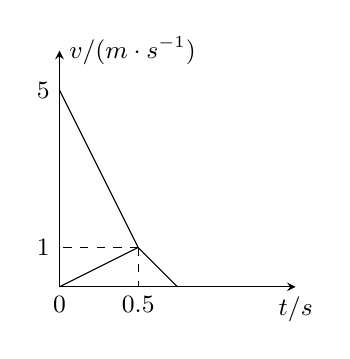
\begin{tikzpicture}
  \draw[->,>=stealth] (0,0) node [anchor=north] {\small 0}--(3,0) node [anchor=north] {\small $t/s$};
  \draw[->,>=stealth] (0,0) --(0,3) node [anchor=west] {\small $v/(m\cdot s^{-1})$};
  \draw (1,0.5)--(1.5,0);
  \draw (1,0.5)--(0,2.5) node [anchor=east]{\small $5$};
  \draw[dashed] (1,0.5)--(0,0.5) node [anchor=east]{\small $1$};
  \draw[dashed](1,0.5)--(1,0) node [anchor=north]{\small $0.5$};
  \draw(1,0.5)--(0,0);
\end{tikzpicture}
:>所示.由加速度的定义,可得
\[
  a=\frac{\Delta v}{\Delta t}=2m/s^2
\]
对物块受力分析,由牛顿第二定律可得
\[
  \mu mg =ma
\]
解得
\[
  \mu =\frac{a}{g}=0.2
\]

ee.(2)物块相对于木板的位移,可以按照匀变速直线运动直接求解,然而在此题中给出了$v-t$图像,直接根据图像分析则更加简洁.在$0.5s$前二者存在相对位移,$0.5s$之后不再发生相对滑动,所以相对位移大小对应<:
\begin{tikzpicture}
  \draw[->,>=stealth] (0,0) node [anchor=north] {\small 0}--(3,0) node [anchor=north] {\small $t/s$};
  \draw[->,>=stealth] (0,0) --(0,3) node [anchor=west] {\small $v/(m\cdot s^{-1})$};
  \draw (1,0.5)--(1.5,0);
  \draw (1,0.5)--(0,2.5) node [anchor=east]{\small $5$};
  \draw[dashed] (1,0.5)--(0,0.5) node [anchor=east]{\small $1$};
  \draw[dashed](1,0.5)--(1,0) node [anchor=north]{\small $0.5$};
  \draw(1,0.5)--(0,0);
  \draw[pattern=north west lines](0,0)--(1,0.5)--(0,2.5);
\end{tikzpicture}
:>中阴影的面积.由几何关系可得
\[
  \Delta x=\frac{1}{2}\times 5 \times 0.5 m=1.25m
\]

4.一长木板置于粗糙水平地面上,木板左端放置一小物块;在木板右方有一墙壁,木板右端与墙壁的距离为$4.5m$,如<:
\begin{tikzpicture}
  \draw[color=white,pattern=north west lines] (-2,0) rectangle (2.2,-0.2); 
  \draw[color=white,pattern=north west lines] (2,0) rectangle (2.2,1); 
  \draw (-2,0)--(2,0);
  \draw (2,0)--(2,1);
  \draw (-1.5,0) rectangle (1,0.2);
  \filldraw (-1.5,0.2) rectangle (-1.3,0.4);
  \draw (0,-0.2) node [anchor=north] {\small (a)};
  \draw[->,>=stealth] (3,0) node [anchor=east]{\small 0}--(6,0) node [anchor=north]{\small $t/s$};
  \draw[->,>=stealth] (3,0) --(3,3) node [anchor=west]{\small $v/(m\cdot s^{-1})$};
  \draw[dashed] (3,2) node [anchor=east]{\small $4$}--(4,2);
  \draw[dashed] (4,2)--(4,0) node [anchor=north] {\small $1$};
  \draw (4,2)--(5,0) node [anchor=north]{\small $2$};
  \draw (3,1) node [anchor=east]{\small $2$}--(3.1,1);
  \draw (4.5,-0.2) node [anchor=north]{\small (b)};
\end{tikzpicture}
:>中(a)所示,$t=0s$时刻开始,小物块与木板一起以共同的速度向右运动,直到$t=1s$时木板与墙壁碰撞(碰撞时间极短).碰撞前后木板速度大小不变,方向相反;运动过程中小物块始终未离开木板.已知碰撞后$1s$时间内小物块的$v-t$图线如(b)所示.木板的质量是小物块质量的$15$倍,重力加速度大小$g$取$10m/s^2$.求:
[1]木板与地面间的动摩擦因数$\mu_1$及小物块与木板间的动摩擦因数$\mu_2$;
[2]木板的最小长度;
[3]木板右端离墙壁的最终距离.

a.见解析

e.(1)选择初速度方向为正,在$0\sim 1s$内,板块一块以相同的加速度匀减速直线运动,由$v-t$图像可得,木板与墙相碰撞前的速度为$v=4m/s$.由运动学平均速度与位移关系得
\[
  x_1=\frac{v_0+v_1}{2}t_1
\]
解得
\[
  v_0=\frac{2x_1}{t_1}-v_1=5m/s
\]
由加速度的定义可得
\[
  a=\frac{v_1-v_0}{t_1}=-1m/s^2
\]
由受力分析及牛顿第二定律可得
\[
  a=-\mu_1 g
\]
解得
\[
  \mu_1 =-\frac{a}{g}=0.1
\]
在$1\sim 2s$内,物块做匀减速直线运动,据加速度定义,由$v-t$图像可得
\[
  a_2=\frac{\Delta v}{\Delta t}=-4m/s^2
\]
对物块受力分析,由牛顿第二定律可得
\[
  a_2=-\mu_2 g
\]
解得
\[
  \mu_2=-\frac{a_2}{g}=0.4
\]

ee.(2)当木板与墙碰撞的瞬间木板的速度为$-4m/s$,木块的瞬时速度为$4m/s$,所以选择木板为参考系时,木块相对于木板的初速度为
\[
u_0=4-(-4)m/s=8m/s
\]
由牛顿第二定律和受力分析易得二者发生相对运动时的加速度分别为木块$a_2=-4m/s^2$ 和木板 $a_1=\frac{4}{3}m/s^2$,所以木块相对于木板的加速度为
\[
  a=-4-\frac{4}{3}m/s^2=-\frac{16}{3}m/s^2
\]
现在来计算达到共同速度,即相对速度为$0$时,所经历的时间.
\[
0=u_0+at
\]
解得
\[
  t=-\frac{u_0}{a}=1.5s
\]
但是这里需要注意,虽然计算出了这个时间,但是不一定能保证木板一直相对于地面运动,所以这时间内要确定木板的运动状态.如果在$1.5s$时计算得出的木板的速度为正,说明板块下一步将继续向右运动,碰撞墙壁后再重复运动过程,最后停在墙壁处,如果计算得出的木板速度为负,说明板块将以相同的速度向左运动,最后停止在远离墙壁的某处.在相对于地的绝对参考系中
\[
  v_2=-4+\frac{4}{3}\times \frac{3}{2}m/s=-2m/s
\]
上式表明木板在$1.5s$时仍然向左运动,也就是说板块的运动是先达到共速再以相同的速度匀减速运动,直到停止.则,当相对速度为$0$时,二者不再发生相对滑动,因此木板的最小长度也就是相对运动的相对位移大小
\[
  L_{min}=\frac{0-u_0^2}{2a}=6m
\]

ee.(3)下面计算木板从碰撞墙壁到最后停止这段时间内的位移,它的大小就是最后木板离墙壁的距离.
\[
  x=\frac{-2+(-4)}{2}\cdot \frac{3}{2}-\frac{(-2)^2}{2}=-6.5m
\]
即:木板右端离墙壁的最终距离为$6.5m$.

\end{calculate}

\section{传送带模型}

\begin{calculate}
 1.如<:
 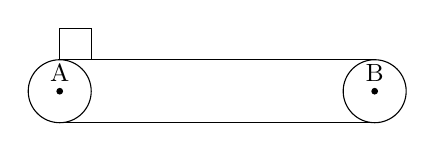
\begin{tikzpicture}
   \draw (-2,0) circle [radius=0.4]; 
   \filldraw[color=black] (-2,0) circle [radius=1pt];
   \draw (-2,0) node [anchor=south]{\small A};
   \draw (2,0) circle [radius=0.4]; 
   \filldraw[color=black] (2,0) circle [radius=1pt];
   \draw (2,0) node [anchor=south]{\small B};
   \draw (-2,0.4)--(2,0.4);
   \draw (-2,-0.4)--(2,-0.4);
   \draw (-2,0.4) rectangle (-1.6,0.8);
 \end{tikzpicture}
 :>所示为一水平传送带装置示意图,绷紧的传送带$AB$始终保持$v=1m/s$的恒定速率运动,一质量为$m=4kg$的行李(可视为质点)无初速度地放在$A$处,传送带对行李的滑动摩擦力使行李开始做匀加速直线运动,随后行李又以与传送带相等的速率做匀速直线运动.设行李与传送带之间的动摩擦因数$\mu=0.1$,$A$、$B$间的距离$l=2m$,$g$取$10m/s^2$.求:
 [1]行李刚开始运动时所受的滑动摩擦力大小与加速度大小;
 [2]行李做匀加速直线运动的时间;
 [3]如果提高传送带的运行速率,行李就能被快速地传送到$B$处.求行李从$A$到$B$处的最知时间和传送带的最小运行速率.

 a.见解析

 e.(1)行李刚开始运动时,对行李受力分析如
<:
 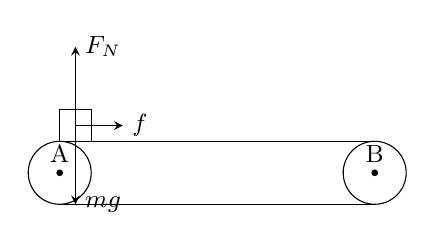
\begin{tikzpicture}
   \draw (-2,0) circle [radius=0.4]; 
   \filldraw[color=black] (-2,0) circle [radius=1pt];
   \draw (-2,0) node [anchor=south]{\small A};
   \draw (2,0) circle [radius=0.4]; 
   \filldraw[color=black] (2,0) circle [radius=1pt];
   \draw (2,0) node [anchor=south]{\small B};
   \draw (-2,0.4)--(2,0.4);
   \draw (-2,-0.4)--(2,-0.4);
   \draw (-2,0.4) rectangle (-1.6,0.8);
   \draw[->,>=stealth] (-1.8,0.6)--+(0,-1) node [anchor=west]{\small $mg$};
   \draw[->,>=stealth] (-1.8,0.6)--+(0,1) node [anchor=west]{\small $F_N$};
   \draw[->,>=stealth] (-1.8,0.6)--+(0.6,0) node [anchor=west]{\small $f$};
 \end{tikzpicture}
:>所示.竖直方向受力平衡得
\[
  F_N-mg=0
\]
解得
\[
  F_N=mg
\]
由$f=\mu F_N$得
\[
  f=\mu mg=4N
\]
由牛顿第二定律得
\[
  f=ma
\]
解得
\[
  a=\frac{f}{m}=1m/s^2
\]

ee.(2)由运动学公式得
\[
  t=\frac{v}{a}=1s
\]

ee.(3)当提高皮带的运行速率,行李能够被较快的传送到$B$处.当皮带速度使行李从$A$到$B$一直做匀加速直线运动时,这个时间最短,即
\[
  l=\frac{1}{2}at_{min}^2
\]
解得
\[
  t_{min}=\sqrt{\frac{2l}{a}}=2s
\]
当行李到$B$时,恰好等于皮带的速度时,这时皮带的速度是保证行李一直做匀加速直线运动的最低运行速率.由运动学公式得
\[
  v_{min}^2=2al
\]
解得
\[
  v_{min}=\sqrt{2al}=2m/s
\]

ee.本题也可以从纯数学的角度来考虑问题.写出行李从$A$到$B$所用的时间$t$和皮带速度$v$的关系
\[
  t=\frac{v}{a}+\frac{l-\frac{v^2}{2a}}{v}
\]
整理后得
\[
  t=\frac{v}{2a}+\frac{l}{v}
\]
由均值不等式$a+b\geq 2\sqrt{ab}$得
\[
  t\geq 2\sqrt{\frac{v}{2a}\cdot \frac{l}{v}}=2\sqrt{\frac{l}{2a}}=2s
\]
上式当且仅当
\[
  \frac{v}{2a}=\frac{l}{v}
\]
时取等,由此解得最小运行速率为
\[
  v_{min}=\sqrt{2al}=2m/s
\]

2.如<:
\begin{tikzpicture}
  \draw (0,0.3) circle [radius=0.3]; 
  \filldraw (0,0.3) circle [radius=1pt]; 
  \draw[color=white,pattern=north west lines] (-1,0) rectangle (1,-0.2);
  \draw (-1,0)--(1,0);
  \draw (0,0.3)++(307:0.3)--+(37:4);
  \draw (0,0.3)++(127:0.3) node [anchor=east]{\small B}--+(37:4) node [anchor=south west]{\small A};
  \draw (0,0.3)++(37:4) circle [radius=0.3];
  \filldraw (0,0.3)++(37:4) circle [radius=1pt];
  \draw [rotate around={37:(0,0.3)}] (3.7,0.6) rectangle (4,0.9);
  \draw (0.4,0) arc (0:37:0.3);
  \draw (18:0.6) node {\small $\theta$};
\end{tikzpicture}
:>所示,传送带与水平地面的夹角为$\theta=37^\circ$,$AB$的长度为$64m$,传送带以$20m/s$的速度沿逆时针方向转动,在传送带上端$A$点无初速度地放上一个质量为$8kg$的物体(可视为质点),它与传送带之间的动摩擦因数为$\mu=0.5$,求物体从$A$点运动到$B$点所用的时间.($\sin 37^\circ =0.6,\cos37^\circ=0.8,g=10m/s^2$)

a.见解析

e.由于$\tan 37^\circ >\mu$,所以在皮带运动过程中不会相对于皮带静止.假设皮带足够长,则物体开始的速度比皮带的速度小,所以物体所受摩擦力方向沿皮带向下;当物体加速到与皮带的速度相同之后,继续加速,所心之后速度就大于皮带的速度,则物体所受摩擦力方向沿皮带向上.这两种情况,受力分析如<:
\begin{tikzpicture}
  \draw (0,0.3) circle [radius=0.3]; 
  \filldraw (0,0.3) circle [radius=1pt]; 
  \draw[color=white,pattern=north west lines] (-1,0) rectangle (1,-0.2);
  \draw (-1,0)--(1,0);
  \draw (0,0.3)++(307:0.3)--+(37:4);
  \draw (0,0.3)++(127:0.3) node [anchor=east]{\small B}--+(37:4) node [anchor=south west]{\small A};
  \draw (0,0.3)++(37:4) circle [radius=0.3];
  \filldraw (0,0.3)++(37:4) circle [radius=1pt];
  \draw [rotate around={37:(0,0.3)}] (3.7,0.6) rectangle (4,0.9);
  \draw [rotate around={37:(0,0.3)}] (2.7,0.6) rectangle (3,0.9);
  \draw [rotate around={37:(0,0.3)}] (1.7,0.6) rectangle (2,0.9);
  \draw [rotate around={37:(0,0.3)}] (1.7,0.9) node [anchor=south]{\small C}; 
  \draw [rotate around={37:(0,0.3)}] (0.7,0.6) rectangle (1,0.9);
  \draw (0.4,0) arc (0:37:0.3);
  \draw (18:0.6) node {\small $\theta$};
  \filldraw (0,0.3)++(127:0.45)++(37:2.85) circle [radius=1pt];
  \draw[->,>=stealth](0,0.3)++(127:0.45)++(37:2.85)--+(0,-0.8) node [anchor=west]{\small $mg$}; 
  \draw[->,>=stealth](0,0.3)++(127:0.45)++(37:2.85)--+(127:0.8) node [anchor=west]{\small $F_N$}; 
  \draw[->,>=stealth](0,0.3)++(127:0.45)++(37:2.85)--+(217:0.4) node [anchor=west]{\tiny $f$}; 
  \draw[->,>=stealth](0,0.3)++(127:0.45)++(37:2.85)--+(217:1) node [anchor=east]{\small $x$}; 
  \draw (0,0.3)++(127:0.45)++(37:2.85)--+(37:1.5); 
  \draw[->,>=stealth](0,0.3)++(127:0.45)++(37:2.85)--+(127:1.2) node [anchor=west]{\small $y$}; 
  \draw(0,0.3)++(127:0.45)++(37:2.85)--+(307:1.5);
  \draw(0,0.3)++(127:0.45)++(37:2.85)++(270:0.3) arc (270:307:0.3);
  \draw(0,0.3)++(127:0.45)++(37:2.85)++(300:0.25)node [anchor=north]{\tiny $\theta$}; 
  \filldraw (0,0.3)++(127:0.45)++(37:0.85) circle [radius=1pt];
  \draw[->,>=stealth](0,0.3)++(127:0.45)++(37:0.85)--+(0,-1) node [anchor=west]{\small $mg$}; 
  \draw[->,>=stealth](0,0.3)++(127:0.45)++(37:0.85)--+(127:0.8) node [anchor=west]{\small $F_N$}; 
  \draw[->,>=stealth](0,0.3)++(127:0.45)++(37:0.85)--+(37:0.5) node [anchor=west]{\small $f$}; 
  \draw[dashed](0,0.3)++(127:0.45)++(37:2.85)++(0,-0.8)--+(37:0.48) node [anchor=south west] {\tiny $mg\sin\theta$}; 
  \draw[dashed](0,0.3)++(127:0.45)++(37:2.85)++(0,-0.8)--+(127:0.64) node [anchor=south east] {\tiny $mg\cos\theta$}; 
  \draw[->,>=stealth](0,0.3)++(127:0.45)++(37:2.85)--+(307:0.64);
  \draw[->,>=stealth](0,0.3)++(127:0.45)++(37:2.85)--+(217:0.48);
\end{tikzpicture}
:>所示,当物块到达$C$处时与皮带达到共同速度,则在$AC$之间受力分析,并正交分解,由$y$轴受力平衡得
\[
  F_N-mg\cos\theta=0
\]
解得
\[
  F_N=mg\cos\theta
\]
对$x$轴由牛顿第二定律得
\[
  mg\sin\theta + \mu mg\cos\theta = ma_1
\]
解得
\[
  a_1=g(\sin\theta +\mu \cos\theta)=10m/s^2
\]
同理可得\footnote{由于当达到共速后摩擦力方向变成沿皮带向上,所以只需要将摩擦力沿皮带向下的情况的结果里的$\mu$改成$-\mu$就可以了.},共速之后$CB$段的加速度为
\[
  a_1=g(\sin\theta -\mu \cos\theta)=2m/s^2
\]
$AC$段以$a_1$匀加速运动的时间为
\[
  t_1=\frac{v}{a_1}=2s
\]
$AC$的位移为
\[
  x_1=\frac{v^2}{2a_1}=20m
\]
$CB$段的匀加速直线运动的位移为
\[
  x_2=l-x_1=44m
\]
$CB$段以$a_2$匀加速运动的时间可以由匀变速直线运动位移与时间的关系得
\[
  x_2=vt_2+\frac{1}{2}a_2t_2^2
\]
代入数据得
\[
  44=20t_2+t_2^2
\]
简单计算可得
\[
  (t_2+22)(t_2-2)=0
\]
由于$t_2>0$所以取
\[
  t_2=2s
\]
所以得,物块从$A$运动到$B$的总时间为
\[
  t=t_1+t_2=4s
\]

ee.{\bf 讨论:}此题是一道2015年全国卷一的高考题,选择了其中的第二问,原本此题还有第一问,即顺时针转动时求物块由$A$运动到$B$的时间.这种情况下由于物块满足下滑条件$\tan\theta >\mu$,所以物块将以加速度$a_2=2m/s^2$从$A$到$B$一直做匀加速度直线运动,而皮带的转速此时对物块的运动没有影响,所以它就是简单的初速度为零的匀变速直线运动求时间的问题.由位移与时间的关系可得
\[
  l=\frac{1}{2}a_2t^2
\]
解得
\[
  t=\sqrt{\frac{2l}{a_2}}=8s
\]
同时,如果此题目中不满足下滑条件,再来求物块从$A$到$B$的时间,则就转化成了与水平传送带相同的计算.即物块先以$a_1$匀加速,再匀速运动,于是其计算时间的表达式为
\[
  t=\frac{v}{a_1}+\frac{l-x_1}{v}
\]
当然在此题目给出的数据不能这样计算,因为本题是满足下滑条件的,上式是不满足下滑条件时的表达式.

ee.{\bf 特别提醒}同学们的是,老师出此类题目,其目的在于增加计算的难度以考查同学的计算和物理分析能力.如果这道题皮带不够长,即$l<x_1$,则物块将以加速度$a_1$一直做匀加速直线运动,所以这和第二章的运动学公式考查无异,也就达不到考查的目的.因此,一旦出现此类题目,同学们应该马上想到这个最复杂的运动情况,并且通过计算第一段的位移$x_1$作出判断物体先以$a_1$匀加速直线运动,达到共速后再以加速度$a_2$匀加速直线运动,并且据$a_1$的表达式可以快速的同理写出$a_2$的表达式,而节省一半的计算量,这个计算技巧也是需要同学位认真体会的,也是大家在相同的时间内竞赛拉开差距的地方.


\end{calculate}
